\section{Motivation}
\label{sec:motivation}
% \adam{Right now, this is written as motivation for the study.  You may want to consider re-writing this as motivation for the need for aggregated explanations instead... and move the experiment-specific motivation to the experiment section.  This depends if you end up creating a new section for the Design contribution or not.}

Experiments for instance-level explanations typically focus on use cases where the explanation is presented to the user one instance at a time. This is helpful when monitoring the continuous performance of a machine learning model in production. However, it limits one's ability to gather a holistic view of a model's behavior (\ie, a global explanation). Looking at many instances is very time consuming and potentially ineffective. It is not clear whether people can build a coherent understanding of a model by looking at a series of instances: comparison between many instances overloads memory and does not leverage the data compression capabilities of aggregate representations.

The main goal of our study is therefore to explore the idea of aggregating data about many instances and their explanations and verify its effects on model comprehension. More precisely, we want to study the effect of aggregation on what we call ``semantic validation'': the ability of a human to validate the decisions of a model according to his or her knowledge of the domain.

For this purpose, somebody knowledgeable with the domain has to verify that the model and the data are consistent with their mental model and, if necessary, override information coming from statistical aggregates on accuracy. This is an important task, especially for models making critical decisions such as those employed in health care~\cite{Caruana:2015:IMH:2783258.2788613} and security.

A second goal of this study is to better understand how explanations contribute to semantic validation. Explanations typically provide, for each instance, a weight or score that conveys information about how important each feature is, for a given decision, and for a given instance. An important question therefore is to better understand what particular benefits, if any, explanations bring to human validation; whether this is conducted using an instance-level exploration strategy or a more compact aggregation. Our hypothesis is that explanations may bring value if they manage to direct the user's attention to instances and features where biases and mistakes reside.

In summary, our experiment aims at studying the effect of two main factors: \textit{aggregation level}, that is, instances vs. aggregations, and explanations, that is, whether feature weights are present or not.

% Instance-level explanations provide an effective way of focusing the attention of a user towards which features are important for a prediction. If a bias in a data set has a non-negligible effects on the semantic quality of the prediction, then this bias will show up in the set of important features.

% Note, that if the bias was in a feature that is never used by the model it would not affect the model's outcomes.

% However, a big disadvantage of instance-level explanations is that the instances have to be inspected individually. This might result in misleading conclusions as users have to extrapolate their general understanding of the machine learning model from the few instances they have inspected. Aggregating the explanations might be the key for improving semantic validation through instance-level explanations.

% Semantic validation works by detecting biases in the training and / or test data. Therefore, in order to study semantic validation we need ground truth data with known biases. We achieved that by manually creating a bias in an otherwise normal data set and using both to compare the detection of biases.

\section{Design Contribution}
\label{sec:design}
In order to effectively analyze machine learning behavior we allow users to compare subsets of the data set to each other.
These subsets are defined by different combinations of cells in the confusion matrix of the machine learning model.
We selected subsets that help understanding the behavior of the model:

\begin{description}
\item[All.] The full data set is shown and no comparison occurs. This is the initial view of the data.
\item[Ground truth.] By comparing rows of the confusion matrix to each other a user can explore the actual labels of the data.
\item[Predicted labels.] By comparing columns of the confusion matrix to each other a user can explore the predicted labels of the model.
\item[Correctness.] By comparing the diagonals of the confusion matrix to each other a user can explore when the model's prediction is correct or incorrect.
\end{description}

It is thinkable to allow more freedom in selecting subsets to, \eg, compare only errors of a certain predicted label, however, this would increase the complexity of the user interface and a user has to understand when to use each of those subsets in order to be effective.

\begin{figure}[t]
\centering
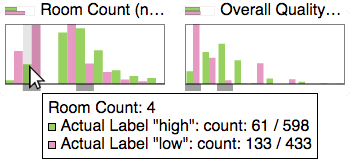
\includegraphics[width=0.7\linewidth]{aggexplain/histogram}
\caption[Comparing the distribution of values by ``Actual Label''.]{
Comparing the distribution of values by ``Actual Label'' (\ie, ground truth).
The height of the bars show the percentage of values within the respective subset (green for ``high'' outcomes and pink for ``low'' outcomes).
The average feature weight of each subset is shown next to the feature name.
This is only visible in the condition including explanations.
}
\label{figs:histogram}
\end{figure}

When aggregating instances, comparing subsets to each other is not trivial.
The na\"ive solution of showing the actual amount of instances with respect to the full data set disadvantages the smaller subset.
However, it is not as important to know the actual distribution, but rather where one subset has a significantly higher or lower concentration of instances compared to the other.
To this extend we propose a novel approach of scaling each subset separately with respect to their own magnitude (see Figure~\ref{figs:histogram}).
Note, that we then compare percentages of instances within the respective subsets.
We further indicate strong differences in the subsets by showing a gray bar at the bottom of the histogram.
We are not aware of any literature that uses or explored this way of comparing subsets with histograms and claim it as a design contribution.
We demonstrate the effectiveness of this design in Section~\ref{sec:results}.

\begin{figure}
\centering
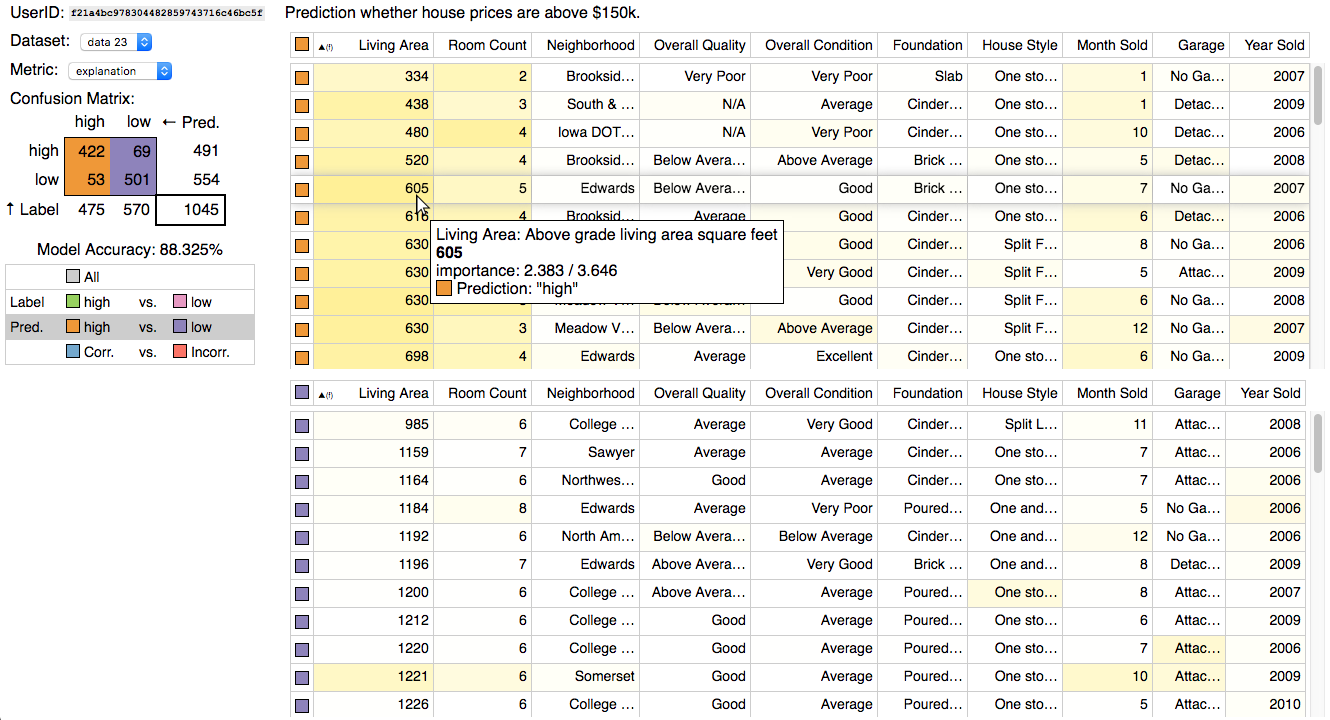
\includegraphics[width=\linewidth]{aggexplain/full_table_expl}
\caption[The full interface illustrating the table view.]{
The full interface illustrating the table view showing individual instances.
The user is comparing the model's prediction of ``high'' house prices (orange) to the prediction of ``low'' prices (purple).
The feature ``Living Area'' is ordered by ascending values and the user hovers over the cell with the value ``605''.
}
\label{figs:full_view}
\end{figure}
